\chapter{Symmetrien der Geradenkonfiguration} \label{chap:configsymm}
Die hohe Zahl an Geraden auf \textsc{Fermat}-Flächen legt es nahe, dass ihre Struktur durch die Geraden in hohem Maß festgelegt wird. Hier wollen wir den Zusammenhang untersuchen zwischen semilinearen Symmetrien der Fläche und Permutationen der Geraden, die das Schnittverhalten respektieren.

Wir führen für dieses Kapitel neue Notation ein: den Primkörper von $K$ bezeichnen wir als $k$. Ohne Einschränkung sei $K = \overline k$ angenommen, denn offenbar sind alle Geraden über $K$ definiert.

\section{Lineare und Kombinatorische Symmetrien}
Die Fermat-Flächen haben einen hohen Grad an Symmetrie. Offenbar lassen sowohl Permutationen der Koordinaten als auch Multiplikation der Koordinaten mit $d$-ten Einheitswurzeln die Fläche invariant. Das sind alles lineare Transformationen, diese reichen aber nicht, um alle Symmetrien der Geradenkonfiguration zu erklären. Dazu müssen wir noch die Automorphismengruppe von $K$ hinzunehmen. Also operieren die Gruppen $S_4$, $\Gal K/k$ und $\mu_d^4$, in letzterer operiert eine Untergruppe isomorph zu $\mu_d$ trivial: Multiplikation aller Koordinaten mit derselben Einheitswurzel ändert nichts. Die Gruppen schneiden sich nur in $\{\id\}$, also haben wir eine Aktion von
\begin{equation}
\mu_d^4 / \mu_d \rtimes (S_4 \times \Gal K/k) \subset \PGaL 4K,
\end{equation}
auf $F_d$, wobei der Homomorphismus $S_4 \times \Gal K/k \rightarrow \Aut(\mu_d^4 / \mu_d)$ so definiert ist: $(\sigma, \tau)$ wird abgebildet auf $\mu_d^4 / \mu_d \to \mu_d^4 / \mu_d$, $(x_0:\dots:x_3) \mapsto (\tau(x_{\sigma(0)}):\dots:\tau(x_{\sigma(3)}))$. Wenn es Geistergeraden gibt, treten sogar noch mehr Symmetrien auf, wie wir später sehen werden.

\begin{defin}
Sei $S \in \proj n(K)$ eine beliebige Menge. Als semilineare Symmetriegruppe von $S$ bezeichnen wir die Untergruppe
\begin{equation}
G_l = G_l(S) = \{ g \in \PGaL{n+1}K: gS = S \} \subset \PGaL{n+1}K.
\end{equation}
\end{defin}

Solche semilinearen Abbildungen lassen nicht nur die Fläche invariant, sondern schicken auch Geraden auf Geraden. Damit permutieren sie die Geraden auf der Fläche, offenbar bleibt dabei aber ihre Schnittkonfiguration erhalten. Die Schnittkonfiguration wird durch einen Graphen $\mathcal G = (L,E)$ kodiert, dabei ist die $L$ die Menge der Geraden, und $(l_1, l_2) \in E$, wenn $l_1$ und $l_2$ sich schneiden.

Die Frage liegt nahe, welche Permutationen der Geraden es denn gibt, die die Schnittkonfiguration erhalten.
\begin{defin}
Sei nun $S \in \proj 3(K)$ eine projektive Fläche, $\mathcal G = (L,E)$ die Geradenkonfiguration. Dann ist die kombinatorische Symmetriegruppe von $S$ die Automorphismengruppe des Graphen $\mathcal G$, d.h.
\begin{equation}
G_k = G_k(S) = \{ \sigma \in \Sym(L): (l_1, l_2) \in E \Leftrightarrow (\sigma(l_1), \sigma(l_2)) \in E \}
\end{equation}
\end{defin}

Wir wollen in diesem Kapitel die Beziehung zwischen diesen beiden Gruppen ausarbeiten. Wie oben bemerkt, induziert jede lineare Symmetrie eine kombinatorische, also haben wir einen Homomorphismus $G_l(F_d) \to G_k(F_d)$. Wir berechnen zunächst den Kern, und zeigen später Surjektivität. Die folgende Betrachtung ist inspiriert durch \cite[Bem.~4.10.1, S.~404]{Hartshorne}, und \cite[Aufg. C--D, S.~180]{Mumford}. Dort wird die Situation für allgemeine reguläre Flächen dritten Grades untersucht.

\begin{lemma}
Gibt es unter den Schnittpunkten der Geraden auf $S$ mindestens fünf in allgemeiner Lage,\footnote{das heißt: keine vier davon liegen auf einer projektiven Ebene.} so besteht der Kern des Homomorphismus $G_l(S) \to G_k(S)$ in einer geeigneten Basis nur aus Automorphismen von $K$.
\end{lemma}
\begin{proof}
Sei $g \in \PGaL 4K$ so gewählt, dass alle Geraden auf $S$ auf sich selbst abgebildet werden. Dann werden auch die fünf Schnittpunkte auf sich selbst abgebildet. Sei $(A, \sigma) \in \GaL 4K = \GL 4K \rtimes \Aut K$ ein Urbild von $g$ und $v_1, \dots, v_5$ Urbilder der Schnittpunke in $K^4$, dann gilt also $(A, \sigma)v_i = \lambda_i v_i$ mit $\lambda_i \in K^*$. Sei $P$ die Matrix mit den Spalten $v_1, \dots, v_4$, dann bildet also $(P^{-1},\id)(A,\sigma)(P,\id) = (P^{-1}AP^\sigma,\sigma)$ die Basisvektoren auf Vielfache ihrer selbst ab. Folglich hat die Matrix $P^{-1}AP^\sigma$ Diagonalgestalt.

Betrachte nun den Vektor $v_5 \in K^4 \setminus 0$ zum fünften Schnittpunkt. In der Basis $\{v_i\}_{i<5}$ hat $v_5$ dann die Gestalt $\sum_i \alpha_i v_i$ mit $\alpha_i \neq 0$ für alle $i$, da die fünf Schnittpunkte in allgemeiner Lage sind. Nun gilt aber $(A,\sigma) v_5 = \lambda_5 v_5$, oder $(P^{-1}AP^\sigma,\sigma)(\alpha_1,\dots,\alpha_4) = \lambda_5(\lambda_1\alpha_1,\dots,\lambda_4\alpha_4)$. Damit sind die Diagonaleinträge $\lambda_1, \dots, \lambda_4$ der Matrix $P^{-1}AP^\sigma$ alle gleich $\lambda$, da die $\alpha_i$ nicht verschwinden. Also ist $P^{-1}AP^\sigma = \lambda \id$, mithin ist $g$ zu $(\id, \sigma)$ linear konjugiert. Man beachte dabei, dass $P$ unabhängig von $g$ ist: man kann also durch einen Basiswechsel alle Elemente des Kerns gleichzeitig auf die Form $(\id, *)$ bringen.
\end{proof}
Wie wir weiter unten sehen werden, schneiden sich zwei Geraden einer Klasse in Punkten der Form $(1:\zeta^n:0:0)$, $\zeta \in \mu_{2d}$ primitiv und $n$ ungerade; sowie Permutationen der Koordinaten. Durch Probieren findet man damit leicht fünf Punkte in allgemeiner Lage. Die fünf $4 \times 4$-Untermatrizen von
\begin{equation*}
\begin{pmatrix}
1 & 0 & 1 & 0 & 1 \\
\zeta & 0 & 0 & 1 & 0 \\
0 & 1 & \zeta^3 & 0 & 0 \\
0 & \zeta & 0 & \zeta^5 & \zeta^3 \\
\end{pmatrix}
\end{equation*}
haben Determinanten $(\zeta^2-1)\zeta^4$, $(\zeta+1)\zeta^4$, $-(\zeta^3+1)\zeta^3$, $-(\zeta^3+1)\zeta^6$ bzw.~$(\zeta+1)\zeta^3$. Für $d>3$ verschwindet keine davon. Im Folgenden nehmen wir die ersten drei Vektoren als Basis.

Nun müssen wir noch ermitteln, welche Automorphismen im Kern liegen. Offenbar gilt im Fall der regulären Geraden $\Gal K/{k(\mu_{2d})} \subset \ker(G_l \to G_k)$, gibt es Geistergeraden, dann $\Gal K/{k(\mu_{d(d-2)})} \subset \ker(G_l \to G_k)$. Wir wollen nun zeigen, dass der Kern nicht größer ist.
\begin{lemma}
Sei $E$ die Körpererweiterung von $k$, die durch die Quotienten der Plückerkoordinaten der Geraden auf der Fläche $S$ erzeugt wird. Der Kern des Homomorphismus $G_l(S) \to G_k(S)$ ist dann $\Gal K/E$.
\end{lemma}
\begin{proof}
Sei die Basis des Raumes wie im vorigen Lemma gewählt, sodass $\ker(G_l \to G_k) \subset \Aut K$. Mit den Geraden sind auch die Schnittpunkte über $E$ definiert, die Verhältnisse der Plückerkoordinaten der transformierten Geraden erzeugen daher auch $E$.

Da diese von einer semilinearen Symmetrie aus dem Kern fix gelassen werden sollen, müssen solche die Verhältnisse der Plückerkoordinaten fix lassen. Damit folgt $\ker(G_l \to G_k) \subset \Gal K/E$. Die Umkehrung ist offensichtlich.
\end{proof}

Damit können wir den Kern explizit angeben: im Fall $d \neq p^n+1$, wenn also keine Geistergeraden existieren, ist $E = k(\mu_{2d})$. Weiter haben wir oben gesehen, dass $\mu_d^4 / \mu_d \rtimes (S_4 \times \Gal K/k) \subset G_l(F_d)$. Nun gilt nach \textsc{Galois}-Theorie
\begin{equation}
\Gal K/k \;/\; \Gal K/{k(\mu_{2d})} \cong \Gal k(\mu_{2d})/k;
\end{equation}
damit folgt, dass $G_k(F_d)$ eine Untergruppe isomorph zu $\mu_d^4 / \mu_d \rtimes (S_4 \times \Gal \mathbb Q(\mu_{2d})/{\mathbb Q})$ enthält. Wir wollen im nächsten Abschnitt zeigen, dass sogar Gleichheit gilt.

\section{Reguläre Geraden}
\paragraph{Konfiguration} Wir schreiben die Geraden aus \eqref{eq:regular} mit einer fixierten primitiven Einheitswurzel $\zeta \in \mu_{2d}$ und $a,b \in (2\mathbb Z + 1)/2d\mathbb Z \subset \Zmod 2dZ$:
\begin{equation}
\begin{split}
\Lcl(I)_{a,b}  :\qquad	&\langle (1,\zeta^a,0,0), (0,0,1,\zeta^b)\rangle \\
\Lcl(II)_{a,b} :\qquad	&\langle (1,0,\zeta^a,0), (0,1,0,\zeta^b)\rangle \\
\Lcl(III)_{a,b}:\qquad	&\langle (1,0,0,\zeta^a), (0,1,\zeta^b,0)\rangle.
\end{split}
\end{equation}
Ob sich zwei verschiedene projektive Geraden schneiden, stellt man anhand der Determinante der Matrix aus ihren vier Basisvektoren fest: verschwindet sie, dann hat die Matrix nicht vollen Rang, also schneiden sie sich in einem projektiven Punkt.

Damit überlegt man sich leicht, dass sich zwei Geraden aus derselben Familie genau dann schneiden, wenn sie in einem der beiden Parameter $a$, $b$ übereinstimmen. Für Geraden aus verschiedenen Klassen ergibt sich folgendes: zwei Geraden $\Lcl(I)_{a,b}$ und $\Lcl(II)_{a',b'}$ schneiden sich, wenn
\begin{equation}
\det \begin{pmatrix}
1 & \zeta^a & 0 & 0 \\
0 & 0 & 1 & \zeta^b \\
1 & 0 & \zeta^{a'} & 0 \\
0 & 1 & 0 & \zeta^{b'}
\end{pmatrix} = 0 \quad\Longleftrightarrow\quad \zeta^{a'} \zeta^b = \zeta^a \zeta^{b'} \quad\Leftrightarrow\quad a-b \equiv a'-b' \pmod{2d}.
\end{equation}
Analog erhält man, dass sich $\Lcl(I)_{a,b}$ und $\Lcl(III)_{a'',b''}$ schneiden, wenn $a''-b'' \equiv a+b$, und $\Lcl(II)_{a',b'}$ und $\Lcl(III)_{a'',b''}$, wenn $a''+b'' \equiv a'+b' \pmod{2d}$.

Wir wollen zur Beschreibung der Schnittkonfiguration noch einige Begriffe einführen: die drei Teilmengen von Geraden $\Lcl(I)$, $\Lcl(II)$ und $\Lcl(III)$ wollen wir Klassen nennen. Die Teilmengen davon mit konstantem Parameter $b$ nennen wir Zeilen, die mit konstantem Parameter $a$ Spalten. Dann bilden die Zeilen und Spalten vollständige Graphen $K_d$.

Teilmengen der Klassen mit konstanter Summe bzw. Differenz der Parameter $a$, $b$ mögen Diagonalen heißen. Bestimmte Diagonalen verschiedener Klassen bilden bipartite Graphen $K_{d,d}$. In der folgenden Grafik sind einige dieser Diagonalen dargestellt. Jede Gerade in einer der Diagonalen schneidet jede andere in der Diagonalen gleicher Farbe in der entsprechenden anderen Klasse.

\begin{figure}[h]
\centering
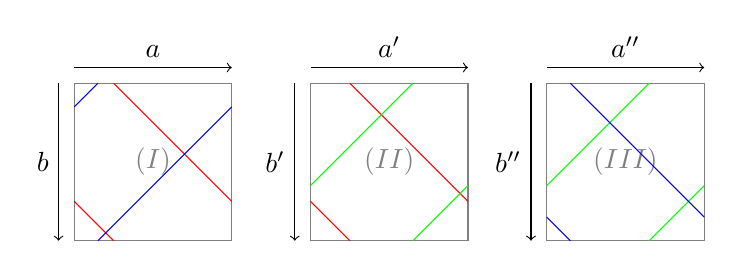
\begin{tikzpicture}
\draw[color=gray]
	[xshift=0cm] (0,0) rectangle (2,2) (1,1) node{$\Lcl(I)$}
	[xshift=3cm] (0,0) rectangle (2,2) (1,1) node{$\Lcl(II)$}
	[xshift=3cm] (0,0) rectangle (2,2) (1,1) node{$\Lcl(III)$};
\draw[->,xshift=0cm] (0,2.2) -- (2,2.2) node[above,midway] {$a$};
\draw[->,xshift=0cm] (-0.2,2) -- (-0.2,0)  node[left,midway] {$b$};
\draw[->,xshift=3cm] (0,2.2) -- (2,2.2) node[above,midway] {$a'$};
\draw[->,xshift=3cm] (-0.2,2) -- (-0.2,0)  node[left,midway] {$b'$};
\draw[->,xshift=6cm] (0,2.2) -- (2,2.2) node[above,midway] {$a''$};
\draw[->,xshift=6cm] (-0.2,2) -- (-0.2,0)  node[left,midway] {$b''$};
\draw[color=red]
	[xshift=0cm] (0.5,0) -- (0,0.5) (0.5,2) -- (2,0.5)
	[xshift=3cm] (0.5,0) -- (0,0.5) (0.5,2) -- (2,0.5);
\draw[color=green]
	[xshift=3cm] (1.3,0) -- (2,0.7) (0,0.7) -- (1.3,2)
	[xshift=3cm] (1.3,0) -- (2,0.7) (0,0.7) -- (1.3,2);
\draw[color=blue]
	[xshift=0cm] (0,1.7) -- (0.3,2) (0.3,0) -- (2,1.7)
	[xshift=6cm,yscale=-1,yshift=-2cm]
		(0,1.7) -- (0.3,2) (0.3,0) -- (2,1.7);
\end{tikzpicture}
\caption{Schnitte zwischen verschiedenen Klassen der regulären Geraden}\label{fig:reg}
\end{figure}

\paragraph{Symmetrien} Wir haben uns bereits klargemacht, dass wir auf $F_d$ eine Aktion der Gruppe $\mu_d^4 / \mu_d \rtimes (S_4 \times \Gal K/k)$ haben, deren Quotient nach $\Gal K/{k(\mu_{2d})}$ auf der Geradenkonfiguration nichttrivial operiert. Machen wir uns zunächst klar, auf welche Weise das geschieht. Multiplikation der $i$-ten Koordinate mit $\zeta^{s_i}$, $s_i$ gerade, bewirkt offenbar eine Verschiebung der Konfiguration in den einzelnen Klassen, und zwar wie folgt:

\begin{figure}[h]
\centering
\begin{tikzpicture}
\draw[color=black]
	[xshift=0cm] (0,0) rectangle (2,2) (1,1) node{$\Lcl(I)$}
	[xshift=5cm] (0,0) rectangle (2,2) (1,1) node{$\Lcl(II)$}
	[xshift=5cm] (0,0) rectangle (2,2) (1,1) node{$\Lcl(III)$};
\draw[->,xshift=0cm] (0.5,2.2) -- (1.5,2.2) node[above,midway] {$+s_0$};
\draw[->,xshift=0cm] (-0.2,1.5) -- (-0.2,0.5) node[left,midway] {$+s_2$};
\draw[->,xshift=0cm] (1.5,-0.2) -- (0.5,-0.2) node[below,midway] {$+s_1$};
\draw[->,xshift=0cm] (2.2,0.5) -- (2.2,1.5) node[right,midway] {$+s_3$};

\draw[->,xshift=5cm] (0.5,2.2) -- (1.5,2.2) node[above,midway] {$+s_0$};
\draw[->,xshift=5cm] (-0.2,1.5) -- (-0.2,0.5) node[left,midway] {$+s_1$};
\draw[->,xshift=5cm] (1.5,-0.2) -- (0.5,-0.2) node[below,midway] {$+s_2$};
\draw[->,xshift=5cm] (2.2,0.5) -- (2.2,1.5) node[right,midway] {$+s_3$};

\draw[->,xshift=10cm] (0.5,2.2) -- (1.5,2.2) node[above,midway] {$+s_0$};
\draw[->,xshift=10cm] (-0.2,1.5) -- (-0.2,0.5) node[left,midway] {$+s_1$};
\draw[->,xshift=10cm] (1.5,-0.2) -- (0.5,-0.2) node[below,midway] {$+s_3$};
\draw[->,xshift=10cm] (2.2,0.5) -- (2.2,1.5) node[right,midway] {$+s_2$};
\end{tikzpicture}
\caption{Aktion von $\mu_d^4 / \mu_d$ auf der Geradenkonfiguration}\label{fig:coordmult}
\end{figure}

Die \textsc{Galois}-Automorphismen aus dem Quotienten $\Gal {k(\mu_{2d})}/k$ wirken ähnlich: ein Automorphismus $\zeta \mapsto \zeta^t$ mit einer fixierten primitiven Einheitswurzel $\zeta \in \mu_{2d}$ und $t \in (\Zmod 2dZ)^*$ bewirkt eine Multiplikation der Indizes $a$, $b$ einer Klasse mit $t$.

\begin{figure}[h]
\centering
\begin{tikzpicture}
\draw[color=black]
	[xshift=0cm] (0,0) rectangle (2,2) (1,1) node{$\Lcl(I)$}
	[xshift=5cm] (0,0) rectangle (2,2) (1,1) node{$\Lcl(II)$}
	[xshift=5cm] (0,0) rectangle (2,2) (1,1) node{$\Lcl(III)$};
\draw[->>,xshift=0cm] (0.5,2.2) -- (1.5,2.2) node[above,midway] {$\phantom{x} \cdot t$};
\draw[->>,xshift=0cm] (-0.2,1.5) -- (-0.2,0.5) node[left,midway] {$\phantom{x} \cdot t$};

\draw[->>,xshift=5cm] (0.5,2.2) -- (1.5,2.2) node[above,midway] {$\phantom{x} \cdot t$};
\draw[->>,xshift=5cm] (-0.2,1.5) -- (-0.2,0.5) node[left,midway] {$\phantom{x} \cdot t$};

\draw[->>,xshift=10cm] (0.5,2.2) -- (1.5,2.2) node[above,midway] {$\phantom{x} \cdot t$};
\draw[->>,xshift=10cm] (-0.2,1.5) -- (-0.2,0.5) node[left,midway] {$\phantom{x} \cdot t$};
\end{tikzpicture}
\caption{Aktion von $\Gal k(\mu_{2d})/k$ auf der Geradenkonfiguration}\label{fig:galois}
\end{figure}

Die Aktion der Koordinatenpermutation ist schwieriger zu beschreiben. Man kann die drei Matrizen wie in Abb.~\ref{fig:perm} gezeigt auf einen Würfel kleben. Dann entspricht die Aktion der $S_4$ der Drehgruppe des Würfels.

\begin{figure}[h] % we might need transform canvas={...} or sloping and slanting node text (http://tex.stackexchange.com/questions/62038/text-placed-in-pespective-on-3d-object)
\centering
\begin{tikzpicture}[x  = {(0.9659cm,0.25882cm)},
                    y  = {(-0.5cm,0.5cm)},
                    z  = {(0cm,1cm)}, scale = 2]
\begin{scope}[canvas is yx plane at z=0]
  \path[draw=black] (0,0) rectangle (2,2);
  \path[fill=gray!80] (0.5,0.5) rectangle (1.5,1.5);
\end{scope}
\path (0,1,0) -- node[sloped, rotate=180, xslant=-0.6]{$\Lcl(III)$} (2,1,0);
\begin{scope}[canvas is zx plane at y=2]
  \path[draw=black] (0,0) rectangle (2,2);
  \path[fill=gray!80] (0.5,0.5) rectangle (1.5,1.5);
\end{scope}
\path (1,2,0) -- node[sloped, xslant=-0.4]{$\Lcl(I)$} (1,2,2);
\begin{scope}[canvas is zy plane at x=2]
  \path[draw=black] (0,0) rectangle (2,2);
  \path[fill=gray!80] (0.5,0.5) rectangle (1.5,1.5);
\end{scope}
\path (2,0,1) -- node[sloped, xscale=-1, xslant=0.8]{$\Lcl(II)$} (2,2,1);
\begin{scope}[canvas is zx plane at y=0]
  \path[draw=black] (0,0) rectangle (2,2);
  \path[fill=gray!50, fill opacity=0.5] (0.5,0.5) rectangle (1.5,1.5);
\end{scope}
\path (0,0,1) -- node[sloped, xslant=0.3]{$\Lcl(I)$} (2,0,1);
\begin{scope}[canvas is zy plane at x=0]
  \path[draw=black] (0,0) rectangle (2,2);
  \path[fill=gray!50, fill opacity=0.5] (0.5,0.5) rectangle (1.5,1.5);
\end{scope}
\path (0,1,2) -- node[sloped, yscale=-1, xslant=-0.8]{$\Lcl(II)$} (0,1,0);
\begin{scope}[canvas is yx plane at z=2]
  \path[draw=black] (0,0) rectangle (2,2);
  \path[fill=gray!50, fill opacity=0.5] (0.5,0.5) rectangle (1.5,1.5);
\end{scope}
\path (1,2,2) -- node[sloped, rotate=180, xslant=0.5]{$\Lcl(III)$} (1,0,2);
\end{tikzpicture}
\caption{Visualisierung der Aktion von $S_4$ auf der Geradenkonfiguration}\label{fig:perm}
\end{figure}

\paragraph{Vergleich der Symmetriegruppen} Wir zeigen nun, dass diese Symmetrien der Geradenkonfiguration die einzigen sind, die das Schnittverhalten respektieren. Zunächst müssen wir die Konfiguration aber genauer untersuchen.

\begin{lemma}
Sei $d \geq 4$, dann sind die einzigen Subgraphen isomorph zu $K_d$ die aus den Geraden einer Klasse bestehenden, die in einem der beiden Parameter übereinstimmen.
\end{lemma}
\begin{remarks}
Für $d=3$ ist das nicht der Fall: die drei Schnittpunkte der Diagonalen in Abb.~\ref{fig:reg} bilden ebenfalls einen $K_3$. (Die Grafik ist hier etwas irreführend: die Diagonalen schneiden sich für ungerades $d$ nur genau einmal.)
\end{remarks}
\begin{proof}
Sei $l \in L$ eine beliebige Gerade, dann schneidet sie jeweils $d-1$ Geraden in derselben Zeile bzw.~Spalte und jeweils $d$ Geraden in den entsprechenden Diagonalen in den anderen beiden Klassen. Wir wollen nun untersuchen, zu welchen vollständigen Graphen $K_d$ die Gerade $l$ gehört.

Von den $d$ Geraden in anderen Klassen, die $l$ schneiden, kann jeweils nur eine Teil des $K_d$ sein: denn diese schneiden sich untereinander nicht, da die Diagonalen von jeder Zeile und jeder Spalte jeweils nur eine Gerade beinhalten. Weiterhin gibt es keine Schnitte zwischen den Geraden in den anderen Klassen, die $l$ schneiden, und denen in derselben Klasse: denn die Geraden in den anderen Klassen schneiden die aus $l$'s Klasse genau dann, wenn sie in derselben Diagonale wie $l$ liegen. Die Diagonalen durch $l$ und die Zeile und Spalte von $l$ schneiden sich aber nur in $l$.

Da es zwischen den Geraden der Zeile von $l$ und der Spalte von $l$ keine weiteren Schnitte gibt, bleiben also drei Möglichkeiten für vollständige Graphen: die Geraden in der Zeile und Spalte von $l$ bilden jeweils einen $K_d$, und $l$ zusammen mit zwei ausgewählten Schnittpunkten in den anderen Klassen bildet einen $K_3$. Mehr ist aber nicht drin, und für $d \geq 4$ ist das nicht genug. Also sind sind alle auftretenden Subgraphen $K_d$ die Zeilen und Spalten einer Klasse.
\end{proof}
Das nächste Resultat besagt, dass kombinatorische Symmetrien die Partition in die Klassen respektieren.
\begin{lemma}
Sei $d \geq 4$, $\sigma \in G_k$ eine kombinatorische Symmetrie und $l_1, l_2 \in L$ zwei Geraden. Sind $l_1$ und $l_2$ in derselben Klasse, dann auch ihre Bilder $\sigma(l_1)$, $\sigma(l_2)$.
\end{lemma}
\begin{proof}
Das vorige Lemma besagt, dass alle vollständigen Subgraphen $K_d$ vollständig in einer Klasse enthalten sind. Gleichzeitig wissen wir, dass jede Gerade zu zwei solchen Subgraphen gehört. Damit ist dieses Lemma offensichtlich: man setze die symmetrische, reflexive Relation
\begin{equation*}
l_1 \sim l_2 \Longleftrightarrow l_1, l_2 \text{ gehören zu einem gemeinsamen Subgraphen } K_d
\end{equation*}
auf den Geraden transitiv fort, dann sind die Äquivalenzklassen genau die drei Klassen $\Lcl(I)$, $\Lcl(II)$, $\Lcl(III)$. Weil die Relation sich offenbar mit Symmetrien verträgt, bleiben also die drei Klassen invariant.
\end{proof}

Damit haben wir einen Homomorphismus $\pi: G_k \to S_3$, der eine kombinatorische Symmetrie auf die entsprechende Permutation der Klassen schickt. Der Kern besteht dann aus denjenigen Symmetrien, die alle drei Klassen invariant lassen. Sei $\mathcal G'$ der Graph einer Klasse, d.\,h.~ein Graph mit Knotenmenge $((2\mathbb Z+1)/2d\mathbb Z)^2$ und Kanten $(a,b) \sim (a',b') \Longleftrightarrow a=a' \vee b=b'$. Dann gilt offenbar
\begin{equation}
\ker(G_k \to S_3) \subseteq (\Aut \mathcal G')^3.
\end{equation}
Daher liegt es nahe, zunächst $\Aut \mathcal G'$ zu untersuchen. Offenbar können sowohl die Zeilen als auch die Spalten beliebig untereinander permutiert werden, und eine Vertauschung von Zeilen und Spalten (Transposition) ist auch möglich. Wir zeigen jetzt, dass mehr nicht geht.
\begin{lemma}
Betrachte den Subgraph $\mathcal G'$ einer Klasse $\Lcl(I/II/III)$. Sei $\sigma \in \Aut \mathcal G'$, dann bildet $\sigma$ entweder Zeilen auf Zeilen und Spalten auf Spalten ab, oder Zeilen auf Spalten und Spalten auf Zeilen.
\end{lemma}
\begin{proof}
Wir betrachten die Zeile $(2\mathbb Z+1)/2d\mathbb Z \times \{1 + 2d\mathbb Z\}$, ihr Bild ist eine Zeile oder Spalte. Ohne Beschränkung der Allgemeinheit können wir annehmen, dass sie auf sich selbst abgebildet wird. (Sonst transponiere entsprechend und permutiere die Zeilen, das ändert nichts an der Aussage.)

Die Menge der Spalten ist nun $\{\{i + 2d\mathbb Z\} \times (2\mathbb Z+1)/2d\mathbb Z : i \in (2\mathbb Z+1)/2d\mathbb Z\}$. Die Knoten einer Spalte haben die Eigenschaft, dass sie alle mit einem und demselben Knoten in der Zeile $(2\mathbb Z+1)/2d\mathbb Z \times \{1 + 2d\mathbb Z\}$ verbunden sind. Damit sind ihre Bilder alle mit einem und demselben Knoten im Bild der Zeile $(2\mathbb Z+1)/2d\mathbb Z \times \{1 + 2d\mathbb Z\}$ verbunden. Folglich sind die Bilder der Spalten wieder Spalten. Damit werden aber auch die restlichen Zeilen auf Zeilen abgebildet. Was anderes bleibt ihnen ja nicht übrig, da es nur $2d$ vollständige Subgraphen $K_d$ in $\tilde{\mathcal G}$ gibt.
\end{proof}

Man kann also die Automorphismengruppe $\Aut \mathcal G'$ in das Kranzprodukt $S_d^2 \rtimes_{\text{kan.}} S_2$ einbetten. Dabei kodieren die Faktoren $S_d$ jeweils die Permutation der Zeilen bzw.~Spalten untereinander, und der Faktor $S_2$, ob Zeilen und Spalten miteinander vertauscht wurden. Wir wollen ein Element $((\sigma_1, \sigma_2), \tau) \in S_d^2 \rtimes S_2$ dabei so verstehen, dass zuerst $\sigma_1$ die Zeilen und $\sigma_2$ die Spalten permutiert, und dann Zeilen und Spalten vertauscht werden, falls $\tau \neq \id$. Mit den Schnitten zwischen verschiedenen Klassen werden wir das nun auf eine deutlich kleinere Gruppe einschränken.
\begin{prop}
Zwei Geraden einer Klasse liegen auf derselben Diagonale genau dann, wenn sie einander nicht schneiden, aber es mindestens $d$ Geraden gibt, die beide schneiden.
\end{prop}
\begin{proof}
Die eine Richtung ist klar. Seien nun zwei Geraden $l_1$, $l_2$ gegeben mit $l_1 \not\sim l_2$, sodass aber $d$ Geraden $k_1, \dots, k_d \in L$ existieren mit $l_1 \sim k_i \sim l_2$ für $1 \leq i \leq d$. Wegen $l_1 \not\sim l_2$ liegen beide nicht in derselben Zeile oder Spalte, also liegen auch die $k_i$ nicht in derselben Zeile oder Spalte, sie liegen also in anderen Klassen.

Die zu $l_1$, $l_2$ inzidenten Geraden in anderen Klassen liegen auf jeweils parallelen Diagonalen in diesen Klassen. Gemeinsame inzidente Geraden gibt es also nur dann, wenn entsprechende Diagonalen zusammenfallen. Damit liegen aber auch $l_1$, $l_2$ auf einer gemeinsamen Diagonale.
\end{proof}
\begin{coroll}
Damit bilden kombinatorische Symmetrien Diagonalen auf Diagonalen ab.
\end{coroll}
\begin{prop}
Eine Symmetrie $\sigma \in \ker \pi$ schickt Diagonalen in einer Klasse auf zu Ihnen parallele Diagonalen.
\end{prop}
\begin{proof}
Wegen Symmetrie der Klassen können wir annehmen, dass es sich um die rote Diagonale in Klasse $\Lcl(I)$ von Abb.~\ref{fig:reg}, d.\,h. eine Diagonale mit konstanter Differenz $a-b$ handelt. Die Geraden auf dieser Diagonale haben gemeinsame inzidente Geraden in $\Lcl(II)$. Da $\sigma$ die Klassen invariant lässt, gilt dies auch für das Bild der Diagonale. Also handelt es sich um eine zur roten parallele Diagonale.
\end{proof}

\begin{lemma}
Ein Automorphismus des Graphen $\mathcal G'$, der Diagonalen auf dazu parallele Diagonalen schickt, hat die Form $((2\mathbb Z+1)/2d\mathbb Z)^2 \ni (x,y) \mapsto (Cx+D_1, Cy+D_2) \in ((2\mathbb Z+1)/2d\mathbb Z)^2$ oder $(x,y) \mapsto (Cy+D_2, Cx+D_1)$ mit $C \in (\Zmod 2dZ)^*$, $D_1, D_2 \in 2\Zmod 2dZ$.
\end{lemma}
\begin{proof}
Sei also $((\sigma_1, \sigma_2), \tau) \in S_d^2 \rtimes S_2$ ein Automorphismus von $\mathcal G'$ und $\{(a,b) : a-b \equiv c \pmod{2d}\}$ mit $c \in 2\Zmod 2dZ$ eine Diagonale. Dann soll ihr Bild eine dazu parallele Diagonale sein, d.\,h. $\sigma_1(a) - \sigma_2(b) \equiv c' \pmod{2d}$ für alle $(a,b)$ mit $a-b \equiv c \pmod{2d}$. Damit ist $\sigma_2(b) \equiv c' + \sigma_1(a) \equiv c' + \sigma_1(c+b)$, es ergibt sich also $\sigma_2$ aus $\sigma_1$. Subtrahiert man die Gleichungen für $c_1=0$, $c_2=2$, so erhält man
\begin{equation*}
\sigma_1(b+2) - \sigma_1(b) \equiv c_2' - c_1' =: 2C \qquad\Longleftrightarrow\qquad \sigma_1(b+2) \equiv \sigma_1(b) + 2C  \mod{2d}.
\end{equation*}
Man beachte dabei, dass die Differenz $\sigma_1(b+2) - \sigma_1(b)$ gerade ist, damit können wir $c_2' - c_1' = 2C$ setzen.

Damit ist $\sigma_1$ offenbar von der Form $\sigma_1(x) = Cx+D_1$ und $\sigma_2$ entsprechend von der Form $\sigma_2(y) = c' + C(c+y) + D_1 = Cy + (c'+Cc+D_1) = Cy + D_2$, $D_2 := c'+Cc+D_1$. Wegen Bijektivität von $\sigma_{1/2}$ ist $C$ offenbar eine Einheit im Ring $\Zmod 2dZ$. Ebenso sieht man leicht, dass $D_1$ und $D_2$ aus dem Ideal $2\Zmod 2dZ$ stammen.
\end{proof}

Aus den letzten beiden Resultaten folgt, dass sich $\ker \pi$ sogar in das deutlich kleinere Produkt von Gruppen
\begin{equation*}
[(2\Zmod 2dZ)^2 \rtimes_\alpha ((\Zmod 2dZ)^* \times S_2)]^3
\end{equation*}
einbetten lässt. Dabei bildet $\alpha \colon ((\Zmod 2dZ)^* \times S_2) \to \Aut ((2\Zmod 2dZ)^2)$ das Paar $(C,\tau)$ auf $(x_1,x_2) \mapsto (Cx_{\tau(1)},Cx_{\tau(2)})$ ab. Für eine weitere Reduktion der kombinatorischen Symmetriegruppe wollen wir nun die Aktionen auf den einzelnen Klassen miteinander korrelieren. Dazu untersuchen wir zunächst, wie obige Gruppe auf den Diagonalen wirkt.

Die Diagonalen $D_n^{k,l}$ bilden selbst auch einen Graphen: sie zerfallen in drei Klassen, die wir mit $(k,l) \in \{\mathrm{I}, \mathrm{II}, \mathrm{III}\} \times \{+,-\}$ indizieren wollen. Die erste Komponente steht für die Klasse, die zweite dafür, ob die Diagonale durch eine konstante Summe oder eine konstante Differenz der Parameter charakterisiert ist. Weiterhin ist eine Diagonale natürlich durch ebenjene Summe bzw.~Differenz $n \in 2\Zmod 2dZ$ bestimmt. Die Kanten sind dann wie folgt gegeben:
\begin{itemize}
\item $D_n^{\mathrm{I},-} \sim D_n^{\mathrm{II},-}$ für alle $n \in 2\Zmod 2dZ$,
\item $D_n^{\mathrm{I},+} \sim D_n^{\mathrm{III},-}$ für alle $n \in 2\Zmod 2dZ$,
\item $D_n^{\mathrm{II},+} \sim D_n^{\mathrm{III},+}$ für alle $n \in 2\Zmod 2dZ$.
\end{itemize}
Ein Automorphismus des Graphen $\mathcal G$ induziert dann offenbar einen Automorphismus des Diagonalengraphen. Ein Automorphismus aus $\ker \pi$ lässt nach obiger Proposition auch die Klassen $(k,l)$ von Diagonalen invariant. Folglich ist die Aktion von $\ker \pi$ auf den Diagonalen in $S_d^6$. Mit vorigem Lemma können wir das erheblich einschränken.

\begin{lemma}
Eine kombinatorische Symmetrie aus $\ker \pi$ von der Form $(D_1, D_2, C, \tau)^{\{\mathrm{I, II, III}\}} \in [(2\Zmod 2dZ)^2 \rtimes_\alpha ((\Zmod 2dZ)^* \times S_2)]^3$ operiert auf den Diagonalen durch $D_n^{k,l} \mapsto D_{\phi_l^k(n)}^{k,l}$ mit $\phi_+^k(n) = C^k n + D_1^k + D_2^k$ und $\phi_-^k(n) = \sign(\tau^k)(C^k n + D_1^k - D_2^k)$. Dabei ist $\sign$ das Signum einer Permutation, also hier der eindeutige Isomorphismus $S_2 \overrel\to^\sim \{\pm 1\}$.
\end{lemma}
\begin{proof}
Die Symmetrie $(D_1, D_2, C, \tau)^{\{\mathrm{I, II, III}\}}$ lässt sich wie folgt zerlegen: zuerst werden die Parameter $a$ und $b$ einer Klasse $k$ mit dem entsprechenden $C^k$ multipliziert, dann wird auf $a$ das entsprechende $D_1^k$ und auf $b$ das entsprechende $D_2^k$ addiert. Zuletzt werden beide Parameter vertauscht, falls $\tau^k \neq \id$.

Das übersetzt sich in folgende Operationen auf den Diagonalen: die Multiplikation der Parameter $a$, $b$ mit $C^k$ bewirkt offenbar eine Multiplikation der Summe/Differenz $n$ mit $C^k$. Die Verschiebungen von $a$, $b$ um $D_{1/2}^k$ bewirken eine entsprechende Verschiebung der Summe/Differenz um denselben Betrag. Hier muss man nur auf das Vorzeichen achten: Verschiebungen in $a$ wirken sich auf Summe und Differenz positiv aus, Verschiebungen in $b$ auf die Summe positiv, auf die Differenz jedoch negativ.

Zuletzt die Transposition: sie lässt die Diagonalen $D_n^{k,+}$ unangetastet, die Differenz der Diagonalen $D_n^{k,-}$ wird jedoch mit $-1$ multipliziert, daher der Faktor $\sign(\tau)$.
\end{proof}

Da nun ein Automorphismus des Diagonalengraphen die Relationen zwischen den Diagonalen erhält, ergeben sich folgende Gleichungen:
\begin{align*}
D_{\phi_-^\mathrm{I}(n)}^{\mathrm{I},-} &\sim D_{\phi_-^\mathrm{II}(n)}^{\mathrm{II},-}
	&\Longrightarrow\qquad \phi_-^\mathrm{I}(n) &= \phi_-^\mathrm{II}(n) \\
D_{\phi_+^\mathrm{I}(n)}^{\mathrm{I},+} &\sim D_{\phi_-^\mathrm{III}(n)}^{\mathrm{III},-}
	&\Longrightarrow\qquad \phi_+^\mathrm{I}(n) &= \phi_-^\mathrm{III}(n) \\
D_{\phi_+^\mathrm{II}(n)}^{\mathrm{II},+} &\sim D_{\phi_+^\mathrm{III}(n)}^{\mathrm{III},+}
	&\Longrightarrow\qquad \phi_+^\mathrm{II}(n) &= \phi_+^\mathrm{III}(n)
\end{align*}
\begin{prop}
Sei $p = aX+b \in \Zmod nZ[X]$ ein lineares Polynom. Dann verschwindet $p$ auf einem Ideal $m\Zmod nZ$ identisch genau dann, wenn $b=0$ und $a \in \frac n m \Zmod nZ$.
\end{prop}
\begin{proof}
Verschwindet $p$ auf $m\Zmod nZ$, dann auch in $0$: damit ist $b=0$. Mit $0 = p(m) - p(0) = am$ folgt dann $a \in \frac n m \Zmod nZ$. Dass die Bedingungen an die Koeffizienten hinreichend sind, ist offensichtlich.
\end{proof}
Da obige Gleichungen lineare Polynomgleichungen sind, die in $n \in 2\Zmod 2dZ$ identisch erfüllt sind, können wir die also Koeffizienten vergleichen. In der ersten Spalte stehen jeweils die Gleichungen für die linearen Koeffizienten modulo $d$, in der zweiten die für die konstanten Koeffizienten.
\begin{align*}
\sign(\tau^\mathrm{I}) C^\mathrm{I} &\equiv \sign(\tau^\mathrm{II}) C^\mathrm{II}
& \sign(\tau^\mathrm{I}) (D_1^\mathrm{I} - D_2^\mathrm{I}) &= \sign(\tau^\mathrm{II}) (D_1^\mathrm{II} - D_2^\mathrm{II}) \\
C^\mathrm{I} &\equiv \sign(\tau^\mathrm{III}) C^\mathrm{III}
& D_1^\mathrm{I} + D_2^\mathrm{I} &= \sign(\tau^\mathrm{III}) (D_1^\mathrm{III} - D_2^\mathrm{III}) \\
C^\mathrm{II} &\equiv C^\mathrm{III}
& D_1^\mathrm{II} + D_2^\mathrm{II} &= D_1^\mathrm{III} + D_2^\mathrm{III}
\end{align*}
Aus den Gleichungen der ersten Spalte folgt dann durch Einsetzen $C^\mathrm{I} \equiv \sign(\tau^\mathrm{III}) C^\mathrm{III} \equiv \sign(\tau^\mathrm{III}) C^\mathrm{II} \equiv \sign(\tau^\mathrm{III})\sign(\tau^\mathrm{I}) / \sign(\tau^\mathrm{II}) C^\mathrm{I}$, oder $\prod_k \sign(\tau^k) = 1$, da $C^\mathrm{I}$ (auch $\mod d$) invertierbar ist und $\sign$ nach $\{\pm 1\}$ abbildet. Mit anderen Worten: entweder gibt es keine oder zwei Transpositionen.

Für ungerades $d$ ist $\Zmod 2dZ \to \Zmod dZ$ injektiv, folglich gilt dann in der ersten Spalten jeweils Gleichheit. Setzen wir $C := C^\mathrm{II} = C^\mathrm{III}$, dann ist $C^\mathrm{I} = \sign(\tau^\mathrm{III}) C$. Es gibt also für ungerade~$d$ nur einen freien Skalierungsparameter $C \in (\Zmod 2dZ)^*$.

Die Gleichungen der zweiten Spalte bilden nun für feste $\sign(\tau^k)$ ein homogenes lineares Gleichungssystem. Offenbar können wir dieses über $\Zmod dZ$ statt $2\Zmod 2dZ$ lösen. Wir interessieren uns also für den Kern der $(\Zmod dZ)$-Modulhomomorphismen $(\Zmod dZ)^6 \to (\Zmod dZ)^3$,
\begin{equation}
v \mapsto
\begin{pmatrix}
\sign(\tau^\mathrm{I}) & -\sign(\tau^\mathrm{I}) & -\sign(\tau^\mathrm{II}) & \sign(\tau^\mathrm{II}) & 0 & 0 \\
1 & 1 & 0 & 0 & -\sign(\tau^\mathrm{III}) & \sign(\tau^\mathrm{III}) \\
0 & 0 & 1 & 1 & -1 & -1
\end{pmatrix}v.
\end{equation}
Die Matrix lässt sich leicht auf Zeilenstufenform bringen, indem man $\sign(\tau^\mathrm{I})$-mal die erste Zeile von der zweiten subtrahiert. Dann sind die Pivoteinträge offenbar $(2,1,\pm 1)$. Zieht man die dritte Zeile noch $\sign(\tau^\mathrm{III})$-mal von der zweiten ab, erhält man
\begin{equation*}
\begin{pmatrix}
\sign(\tau^\mathrm{I}) & -\sign(\tau^\mathrm{I}) & -\sign(\tau^\mathrm{II}) & \sign(\tau^\mathrm{II}) & 0 & 0 \\
0 & 2 & 0 & -2\sign(\tau^\mathrm{III}) & 0 & 2\sign(\tau^\mathrm{III}) \\
0 & 0 & 1 & 1 & -1 & -1
\end{pmatrix}
\end{equation*}
wegen $\prod_k \sign(\tau^k) = 1$. Als Einheit ist $1$ immer invertierbar; und $2$ ist es genau dann, wenn $d$ ungerade ist. Damit ist der Lösungsraum $(\Zmod dZ)^3$ für ungerades $d$ und $(\Zmod dZ)^3 \times (\frac d2\Zmod dZ) \cong (\Zmod dZ)^3 \times \Zmod 2Z$ für gerades $d$.

\begin{theorem}
Sei $d \geq 4$ ungerade und $\Char K=0$. Dann sind die einzigen Symmetrien der Geradenkonfiguration die durch die semilineare Gruppe erzeugten.
\end{theorem}
\begin{proof}
Wir sahen im vorigen Abschnitt, dass für $\Char K=0$ die kombinatorische Symmetriegruppe eine Gruppe isomorph zu $\mu_d^4 / \mu_d \rtimes (S_4 \times \Gal \mathbb Q(\mu_{2d})/{\mathbb Q})$ enthält. Gerade haben wir eine obere Schranke für $G_k$ hergeleitet: nämlich $[C_d^3 \rtimes (C_2^2 \times (\Zmod 2dZ)^*)] \rtimes S_3$ für ungerades $d$.

Beide haben offenbar dieselbe Anzahl Elemente, man sieht sogar leicht den Isomorphismus wegen $S_4/V_4 \cong S_3$. Damit muss $G_l \to G_k$ surjektiv sein.
\end{proof}

\section{Geistergeraden}
\paragraph{Symmetrien} Es liegen in diesem Fall nicht nur mehr Geraden vor, sondern auch deutlich mehr Symmetrien: es ist seit längerem bekannt, dass hier die unitäre Gruppe $\Unit 4{\mathbb F_{q^2}}$ mit dem Sesquilinearprodukt definiert durch die Konjugation $\overline x = x^q$ operiert.\footcite[siehe u.\,a.][S.~102]{Tate} Diese definiert offenbar einen Körperautomorphismus der Ordnung 2. Die Skalarmatrizen in $\mathbb U(4, \mathbb F_{q^2})$ operieren dabei natürlich trivial: das sind die Matrizen der Form $\lambda \mathbb I$ mit $\lambda \overline{\lambda} = \lambda^{q+1} = 1$, d.\,h. $\lambda \in \mu_d$. Weiterhin operiert natürlich wie im regulären die \textsc{Galois}-Gruppe $\Gal K/k = \Gal \overline{\mathbb F_p}/{\mathbb F_p}$, also insgesamt
\begin{equation}
\Unit 4{\mathbb F_{q^2}}/(\mu_d \mathbb I) \rtimes \Gal \overline{\mathbb F_p}/{\mathbb F_p} \subset G_l(F_d).
\end{equation}
Offenbar liegen die Symmetrien aus dem vorigen Abschnitt auch in der unitären Gruppe: Permutationsmatrizen sind natürlich unitär und Multiplikation einzelner Koordinaten mit Elementen $\lambda \in \mu_d$ auch, da für solche $\lambda \overline{\lambda}=1$ gilt, wie wir gerade festgestellt haben.

\paragraph{Eine Stratifizierung von $F_d(\mathbb F_{q^2})$} Offenbar sind alle Geraden (reguläre und Geistergeraden) über $\mathbb F_p(\mu_{d(d-2)}) = \mathbb F_{q^2}$ mit $q = p^n$, $d = q+1$, definiert. Damit können wir effektiv $F_d(\mathbb F_{q^2})$ betrachten. Insbesondere wollen wir berechnen, wie groß diese (nun endliche) Menge ist. Dazu zerlegen wir zunächst $F_d(K)$ in drei Teile:
\begin{align*}
S_0(K) &= \{\text{alle vier Koord.}\neq 0\} = \{(X,Y,Z,W) \in F_d : XYZW \neq 0\} \\
S_1(K) &= \{\text{genau eine Koord.}= 0\} \\
S_2(K) &= \{\text{genau zwei Koord.}= 0\} = \{\text{mind. zwei Koord.}= 0\} \\
	&= \{X = 0, Y = 0\} \cup \{X = 0, Z = 0\} \cup \dots \cup \{Z = 0, W = 0\}
\end{align*}
Dabei ist $S_0$ offen und $S_2$ abgeschlossen in der Zariski-Topologie auf $F_d$. Jede projektive Gerade besteht aus $q^2+1$ Punkten über $\mathbb F_{q^2}$. Die regulären Geraden liegen in $S_0 \cup S_2$: ist eine Koordinate null, dann auch eine andere. Genauer: es liegen zwei Punkte in $S_2$, die anderen $q^2-1$ in $S_0$.

Die Geistergeraden hingegen liegen in $S_0 \cup S_1$: gäbe es einen Punkt aus $S_2$ darauf, könnte man ihn als Basisvektor nehmen. Dann würde aber eine \textsc{Plücker}-Koordinate verschwinden. Man kann wieder präzisieren: es liegen 4 Punkte in $S_1$ und $q^2-3$ in $S_0$.

Wir wollen nun die Anzahl der Lösungen von $X^d+Y^d+Z^d+W^d=0$ in $\mathbb F_{q^2}$ bestimmen. Dazu bemerken wir zunächst, dass $\lambda^{q+1} \in \mathbb F_q^*$ für $\lambda \in \mathbb F_{q^2}^*$. Andersherum gibt es für jedes $\alpha \in \mathbb F_q^*$ genau $q+1$ verschiedene $\beta \in \mathbb F_{q^2}^*$ mit $\beta^{q+1} = \alpha$. Wir suchen daher Lösungen von $A+B+C+D=0$ in $\mathbb F_q^4$ und liften diese nach $\mathbb F_{q^2}^4$. Dann reduzieren wir sie auf $\proj 3(\mathbb F_{q^2})$.

Für $S_0(\mathbb F_{q^2}) = \{\text{alle vier Koord.}\neq 0\}$ suchen wir also Lösungen von $A+B+C+D=0$ mit $A,B,C,D \in \mathbb F_q^*$. Die ersten beiden Koordinaten $A$, $B$ können wir beliebig wählen. Die vorletzte Koordinate $C$ muss dann so gewählt werden, dass die letzte nicht verschwindet, also $C \neq 0, -A-B$. Für $A+B=0$ fallen beide Fälle zusammen, das passiert $(q-1)$-mal. Damit haben wir
\begin{equation*}
\underbrace{(q-1)(q-2)(q-2)}_{A+B \neq 0} + \underbrace{(q-1)(q-1)}_{A+B=0} = (q-1)((q-2)^2+(q-1))
\end{equation*}
Lösungen. Jede Koordinate hat $(q+1)$ Urbilder unter $x \mapsto x^{q+1}$ in $\mathbb F_{q^2}$. Weil wir uns für Punkte im projektiven Raum interessieren, müssen wir noch durch $\#\mathbb F_{q^2}^* = q^2-1$ teilen und erhalten
\begin{equation}
(q-1)((q-2)^2+(q-1))(q+1)^4/(q^2-1) = ((q-2)^2+(q-1))(q+1)^3
\end{equation}
Punkte in $S_0(\mathbb F_{q^2}) \subset \proj 3(\mathbb F_{q^2})$.

Um die Punkte in $S_1(\mathbb F_{q^2}) = \{\text{genau eine Koord.}= 0\}$ zu zählen, platzieren wir zunächst die Null: dafür gibt es vier Möglichkeiten. Für die restlichen Koordinaten gehen wir wie oben vor: hat man die ersten beiden Koordinaten $A$ und $B$ gewählt, ergibt sich $C=-A-B$. Damit das nicht verschwindet, muss $B$ so gewählt werden, dass $A+B \neq 0$. Also wählt man $A \neq 0$ beliebig und dann $B \neq 0, -A$. Es ergeben sich $4(q-1)(q-2)$ Möglichkeiten. Insgesamt gibt es also in $S_1(\mathbb F_{q^2})$ genau
\begin{equation}
4(q-1)(q-2)(q+1)^3/(q^2-1) = 4(q-2)(q+1)^2 \quad\text{Punkte.}
\end{equation}

Zuletzt zu den Punkten in $S_2(\mathbb F_{q^2}) = \{\text{genau zwei Koord.}= 0\}$. Für die Platzierung der zwei Nullen gibt es zuächst $\binom 4 2 = 6$ Möglichkeiten. Von den zwei verbleibenden Koordinaten legt eine die andere fest, also gibt es $q-1$ Möglichkeiten dafür. Damit haben wir $6(q-1)$ Lösungen in $\mathbb F_q$ und $S_2(\mathbb F_{q^2})$ besteht aus
\begin{equation}
6(q-1)(q+1)^2/(q^2-1) = 6(q+1) \quad\text{Punkten.}
\end{equation}

Zusammengenommen liegen also auf $F_d(\mathbb F_{q^2})$ genau
\begin{equation}
((q-2)^2+(q-1))(q+1)^3 + 4(q-2)(q+1)^2 + 6(q+1) = (q+1)(q^2-q+1)(q^2+1)
\end{equation}
bzw.~$(q^2+1)(q^3+1)$ Punkte. Im letzten Kapitel sahen wir, dass sich auf der Fläche $3d^2 + (d-3)d^3 = 3(q+1)^2 + (q-2)(q+1)^3 = (q+1)(q^3+1)$ Geraden befinden. Jede dieser Geraden besteht aus $q^2+1$ Punkten, das sind insgesamt $(q+1)(q^2+1)(q^3+1)$ Punkte. Also gehen durch jeden Punkt der Fläche im Durchschnitt $q+1$ Geraden.

\paragraph{Die Aktion der unitären Gruppe} Wir wollen nun zeigen, dass durch jeden Punkt genau $q+1$ Geraden gehen. Dazu untersuchen wir, wie die unitäre Gruppe $\mathbb U(4, \mathbb F_{q^2})$ auf der Fläche operiert.\footnote{Den entscheidenden Hinweis für die folgende Argumentation verdanke ich Prof.~David J.~Green.} Offenbar besteht die Fläche genau aus den Vektoren der Norm $0$, genannt \emph{isotrope} Vektoren.
\begin{lemma}
Sei $\alpha \in \mathbb F_{q^2}$ mit $\alpha^{q+1} = -1$ und $v \in \mathbb F_{\!q^2}^{\,n} \setminus \{0\}$ ein Vektor mit $\|v\|^2 = 0$. Dann gibt es ein~$\lambda \in \mathbb F_{q^2}$ und eine Orthonormalbasis $v_1, \dots, v_n$ von $\mathbb F_{\!q^2}^{\,n}$ mit $v = \lambda (v_1 + \alpha v_2)$.
\end{lemma}
\begin{proof}
Wegen $v \neq 0$ gibt es einen Vektor~$v_1$ mit $\lambda = \langle v, v_1 \rangle \neq 0$. Man kann $v_1$ mit einem geeigneten Faktor aus $\mathbb F_{\!q^2}$ multiplizieren, dass $\|v_1\|^2 = 1$ gilt: die Norm nimmt Werte in~$\mathbb F_q$ an und der Homomorphismus $\mathbb F_{\!q^2}^* \to \mathbb F_q^*: x \mapsto x^{q+1}$ hat Kern~$\mu_{q+1}$, also hat das Bild~$q-1$ Elemente, demnach ist er surjektiv. Nehmen wir also an, dass $v_1$ gleich so gewählt wurde.

Dann steht $v - \overline{\lambda} v_1$ orthogonal auf $v_1$ und $\|v - \overline{\lambda} v_1\|^2 = \langle v - \overline{\lambda} v_1, v - \overline{\lambda} v_1 \rangle = \langle v, v \rangle - \lambda \langle v_1, v \rangle - \overline{\lambda} \langle v, v_1 \rangle + \lambda\overline{\lambda} \langle v_1, v_1 \rangle = - \lambda \overline{\lambda} - \lambda \overline{\lambda} + \lambda \overline{\lambda} = -\lambda^{q+1} \in \mathbb F_q$. Damit gilt für den Vektor $v_2 = (\alpha\lambda)^{-1} (v - \overline{\lambda} v_1)$, dass $\|v_2\|^2 = 1$ und $v_2 \perp v_1$. Es gibt also eine Orthonormalbasis, die das Orthonormalsystem~$v_1, v_2$ fortsetzt.

Umstellen der letzten Gleichung ergibt $v = \overline{\lambda} v_1 + \alpha\lambda v_2$. Wegen $\overline{\lambda} = \lambda^q$ können wir $\overline{\lambda} v_1 + \alpha\lambda v_2 = \lambda(\lambda^{q-1} v_1) + \alpha\lambda v_2$ schreiben. Multiplikation mit $\lambda^{q-1}$ ändert die Norm eines Vektors nicht, denn $(\lambda^{q-1})^{q+1} = \lambda^{q^2-1} = 1$. Also können wir $v_1$ in der Orthonormalbasis durch $\lambda^{q-1} v_1$ ersetzen.
\end{proof}

\begin{theorem}
Die projektive unitäre Gruppe $\Unit 4{\mathbb F_{\!q^2}} / (\mu_d \mathbb I)$ operiert auf der Fermat-Fläche $F_d(\mathbb F_{\!q^2}) = \mathbb P(\{v \in \mathbb F_{\!q^2}^{\,4}: \|v\| = 0\})$ transitiv.
\end{theorem}
\begin{proof}
Zunächst überlegen wir uns, dass die unitäre Gruppe auf den Orthonormalbasen des Raumes transitiv operiert: schreibt man die Vektoren einer Orthonormalbasis als Spalten in eine Matrix, erhält man eine unitäre Matrix. Damit liegen alle Orthonormalbasen in der Bahn der Standardorthonormalbasis.

Fixiere nun ein $\alpha \in \mathbb F_{q^2}$ mit $\alpha^{q+1} = -1$. Dann lassen sich nach vorigem Lemma alle Vektoren $v$ mit $\|v\| = 0$ als $\lambda (v_1 + \alpha v_2)$ mit einer Orthonormalbasis $v_1, \dots, v_n$ schreiben. Wie wir eben gesehen haben, operiert auf denen die unitäre Gruppe transitiv, also nach Übergang zum Projektiven auch auf $F_d$.
\end{proof}
\begin{coroll}
Durch jeden Punkt auf $F_d(\mathbb F_{\!q^2})$ gehen genau~$d$ der Geraden, die auf der Fläche~$F_d$ liegen.
\end{coroll}
\begin{proof}
Die projektive unitäre Gruppe lässt die Fläche invariant und permutiert somit die Punkte und die Geraden auf dieser Fläche. Da die Operation auf den Punkten transitiv ist, muss durch jeden Punkt diesselbe Anzahl an Geraden gehen. Nach den Überlegungen aus dem vorigen Abschnitt kann das nur $d=q+1$ sein.
\end{proof}

Mit obigem Lemma können wir uns auch überlegen, dass es nicht mehr als die unitären Symmetrien gibt.
\begin{theorem}
Sei $\phi: \proj 3(\mathbb F_{q^2}) \to \proj 3(\mathbb F_{q^2})$ eine projektive Abbildung, die $F_d(\mathbb F_{q^2})$ invariant lässt. Dann ist $\phi \in \Unit 4{\mathbb F_{q^2}}/(\mu_{q+1} \mathbb I)$.
\end{theorem}
\begin{proof}
Betrachte eine Liftung $\psi$ von $\phi$ nach $\GL 4{\mathbb F_{q^2}}$. Seien $v \perp w$ Vektoren mit $\|v\|^2 = \|w\|^2 = 1$. Da die Norm als Abbildung $\mathbb F_{q^2}^* \to \mathbb F_q^*$ surjektiv ist, können wir anisotrope Vektoren durch Skalierung immer auf Norm $1$ bringen.

Für alle $\alpha$ mit $\alpha^{q+1} = -1$ gilt dann $\|v + \alpha w\|^2 = \|v\|^2 - \|w\|^2 = 0$. Damit folgt $\|\psi(v) + \alpha \psi(w)\|^2 = \| \psi(v) \|^2 + \mathrm{Tr}(\alpha \langle \psi(v), \psi(w) \rangle) - \| \psi(w) \|^2 = 0$. Da dies für alle $\alpha \in \mu_{q+1}$ gilt, die ja $\mathbb F_{q^2}$ als $\mathbb F_q$-Vektorraum erzeugen, und die Spurform nicht entartet ist, folgt $\langle \psi(v), \psi(w) \rangle = 0$. Also folgt, dass $\psi$ Orthogonalität erhält. Setzen wir dies nun wieder ein, ergibt sich $\| \psi(v) \|^2 - \| \psi(w) \|^2 = 0$ oder $\| \psi(v) \|^2 = \| \psi(w) \|^2$.

Also sendet $\psi$ Vektoren gleicher Länge auf Vektoren gleicher Länge: für isotrope Vektoren war das schon gegeben, für die anderen haben wir es gerade gezeigt. Sei $\beta$ eine Quadratwurzel von $\| \psi(v) \|^2 / \|v\|^2 \in \mathbb F_q$ in $\mathbb F_{q^2}$ für einen beliebigen Vektor $v$ mit Norm $\neq 0$: die gibt es immer, da dies die einzige quadratische Erweiterung von $\mathbb F_q$ ist. Weiterhin ist sie verschieden von null, da wegen Bijektivität aus $\|v\|^2 \neq 0$ bereits $\|\psi(v)\|^2 \neq 0$ folgt. Betrachten wir nun $\beta^{-1} \psi$, dann erhält diese Abbildung immer noch Orthogonalität und jetzt auch Normen. Also ist sie unitär noch Fakt~\ref{fact:norminv} und $\phi$ ist ihr Bild in der projektiven unitären Gruppe.
\end{proof}
\begin{coroll}
Die linearen Symmetrien der Fläche $F_{q+1}(\overline{\mathbb F_q})$ sind also genau die projektiv unitären.
\end{coroll}
\begin{proof}
Eine lineare Symmetrie des $\proj 3$ permutiert die Schnittpunkte der Geraden, die über $\mathbb F_{q^2}$ definiert sind. Da diese den Raum aufspannen, wie wir am Anfang des Kapitels gesehen haben, ist also auch die lineare Symmetrie über $\mathbb F_{q^2}$ definiert. Mit dem gerade gezeigten Satz folgt die Aussage.
\end{proof}

\section{Ausblick}
Man könnte das Folgende auch als missglückte Beweisidee verstehen. Sie liefert allerdings einen guten Grund, warum die alle Symmetrien der Geradenkonfiguration durch semilineare Symmetrien der Fläche induziert werden. \note Wollen wir das mit in die Arbeit aufnehmen?

Wir haben gerade gesehen, dass durch jeden Punkt von $F_d(\mathbb F_{q^2})$ im Durchschnitt $q+1$ Geraden gehen. Tatsächlich sind es für jeden Punkt genau so viele, denn die semilineare Symmetriegruppe, die wir im nächsten Abschnitt angeben werden, operiert transitiv auf $F_d(\mathbb F_{q^2})$. Damit muss durch jeden Punkt dieselbe Anzahl an Geraden gehen.

Damit korrespondieren Punkte in $F_d(\mathbb F_{q^2})$ zu vollständigen Subgraphen $K_d = K_{q+1}$ der Schnittkonfiguration: andere vollständige Graphen kann es nicht geben, wie man sich leicht überlegt. Damit induziert eine kombinatorische Symmetrie eine Permutation der Punkte auf $F_d(\mathbb F_{q^2})$. Diese erhält außerdem Geraden: mehrere Punkte liegen nämlich genau dann auf einer Geraden, wenn die dazugehörigen $K_d$ einen Knoten gemeinsam haben. Diese Eigenschaft wird durch Graphautomorphismen erhalten.

Wir haben also eine Abbildung $F_d(\mathbb F_{q^2}) \to F_d(\mathbb F_{q^2})$, die Kollinearität erhält. Nach dem \emph{Fundamentalsatz der projektiven Geometrie}\footnote{siehe bspw.~\cite[S.~72]{Dieudonne}.} ist jede Abbildung $\proj 3(\mathbb F_{q^2}) \to \proj 3(\mathbb F_{q^2})$, die Kollinearität erhält, eine semilineare Abbildung. Da $F_d(\mathbb F_{q^2})$ vollständig von Geraden abgedeckt wird, ist zumindest verständlich, warum der Homomorphismus $G_l \to G_k$ surjektiv ist.
